% !TeX spellcheck = it_IT
\documentclass[11pt, twocolumn]{article}

\usepackage{graphicx}

\newenvironment{myitemize}
{ \begin{itemize}
		\setlength{\itemsep}{0pt}
		\setlength{\parskip}{0pt}
		\setlength{\parsep}{0pt}     }
	{ \end{itemize}                  } 

\newenvironment{myenumerate}
{ \begin{enumerate}
		\setlength{\itemsep}{0pt}
		\setlength{\parskip}{0pt}
		\setlength{\parsep}{0pt}     }
	{ \end{enumerate}                  } 


\title{Technological Infrastructures}
\author{}
\date{}

\begin{document}

\maketitle

\begin{abstract}
L'obiettivo del corso è forninre conoscenza solida delle piattaforme tecnologiche e computing platforms.
Differenza delle responsabilità di Data Scientist e Data Engineer.
Il corso è diviso in 2 parti.
L'esame consiste in 15 domande sia aperte che chiuse per parte e si può arrivare a 30 con lo scritto, si può fare un progetto non obbligatorio che vale al più 3 punti.
\end{abstract}

%\section{Lezione 1 - 02/10}

%\section{Lezione 2 - 08/10}

\section{Componenti di NIST}
NIST sviluppa standard di riferimento per il pubblico. Software Architecture è un organizzazione globale di sistemi software, quindi consiste in:
\begin{myitemize}
	\item divisione della componenti software in sottosistemi; 
	\item Definisce le politiche con cui questi sistemi interagiscono;
	\item definisce le interfacce tra le varie componenti.
\end{myitemize}
Un'architettura di riferimento è essenzialmente un template (scatola vuota con elementi prefissati), fornisce solo il vocabolario usato comunemente per discutere le implementazioni di un dato software.\\
Un'architettura di riferimento per il software non è altro che architettura software dove le strutture e i vari elementi e relazioni sono forniti dai template.
\\
NIST fornisce l'architettura di riferimento per i Big Data che:
\begin{myitemize}
	\item Fornisce un linguaggio comune per i stakeholders;
	\item Incoraggia aderenza ai standard comuni;
	\item Permette di implementare le architetture con una certa consistenza;
	\item Illustra e migliora la comprensione delle componenti, processi e  sistemi di Big Data;
\end{myitemize}

\subsection{I 5 ruoli principali per Big Data}
L'architettura concettuale dei Big Data è un architettura a croce con due assi: Information value (IV) e Information Technology (IT) (Fig \ref{fig:NBDRA}).\\
\begin{figure*}
	\centering
	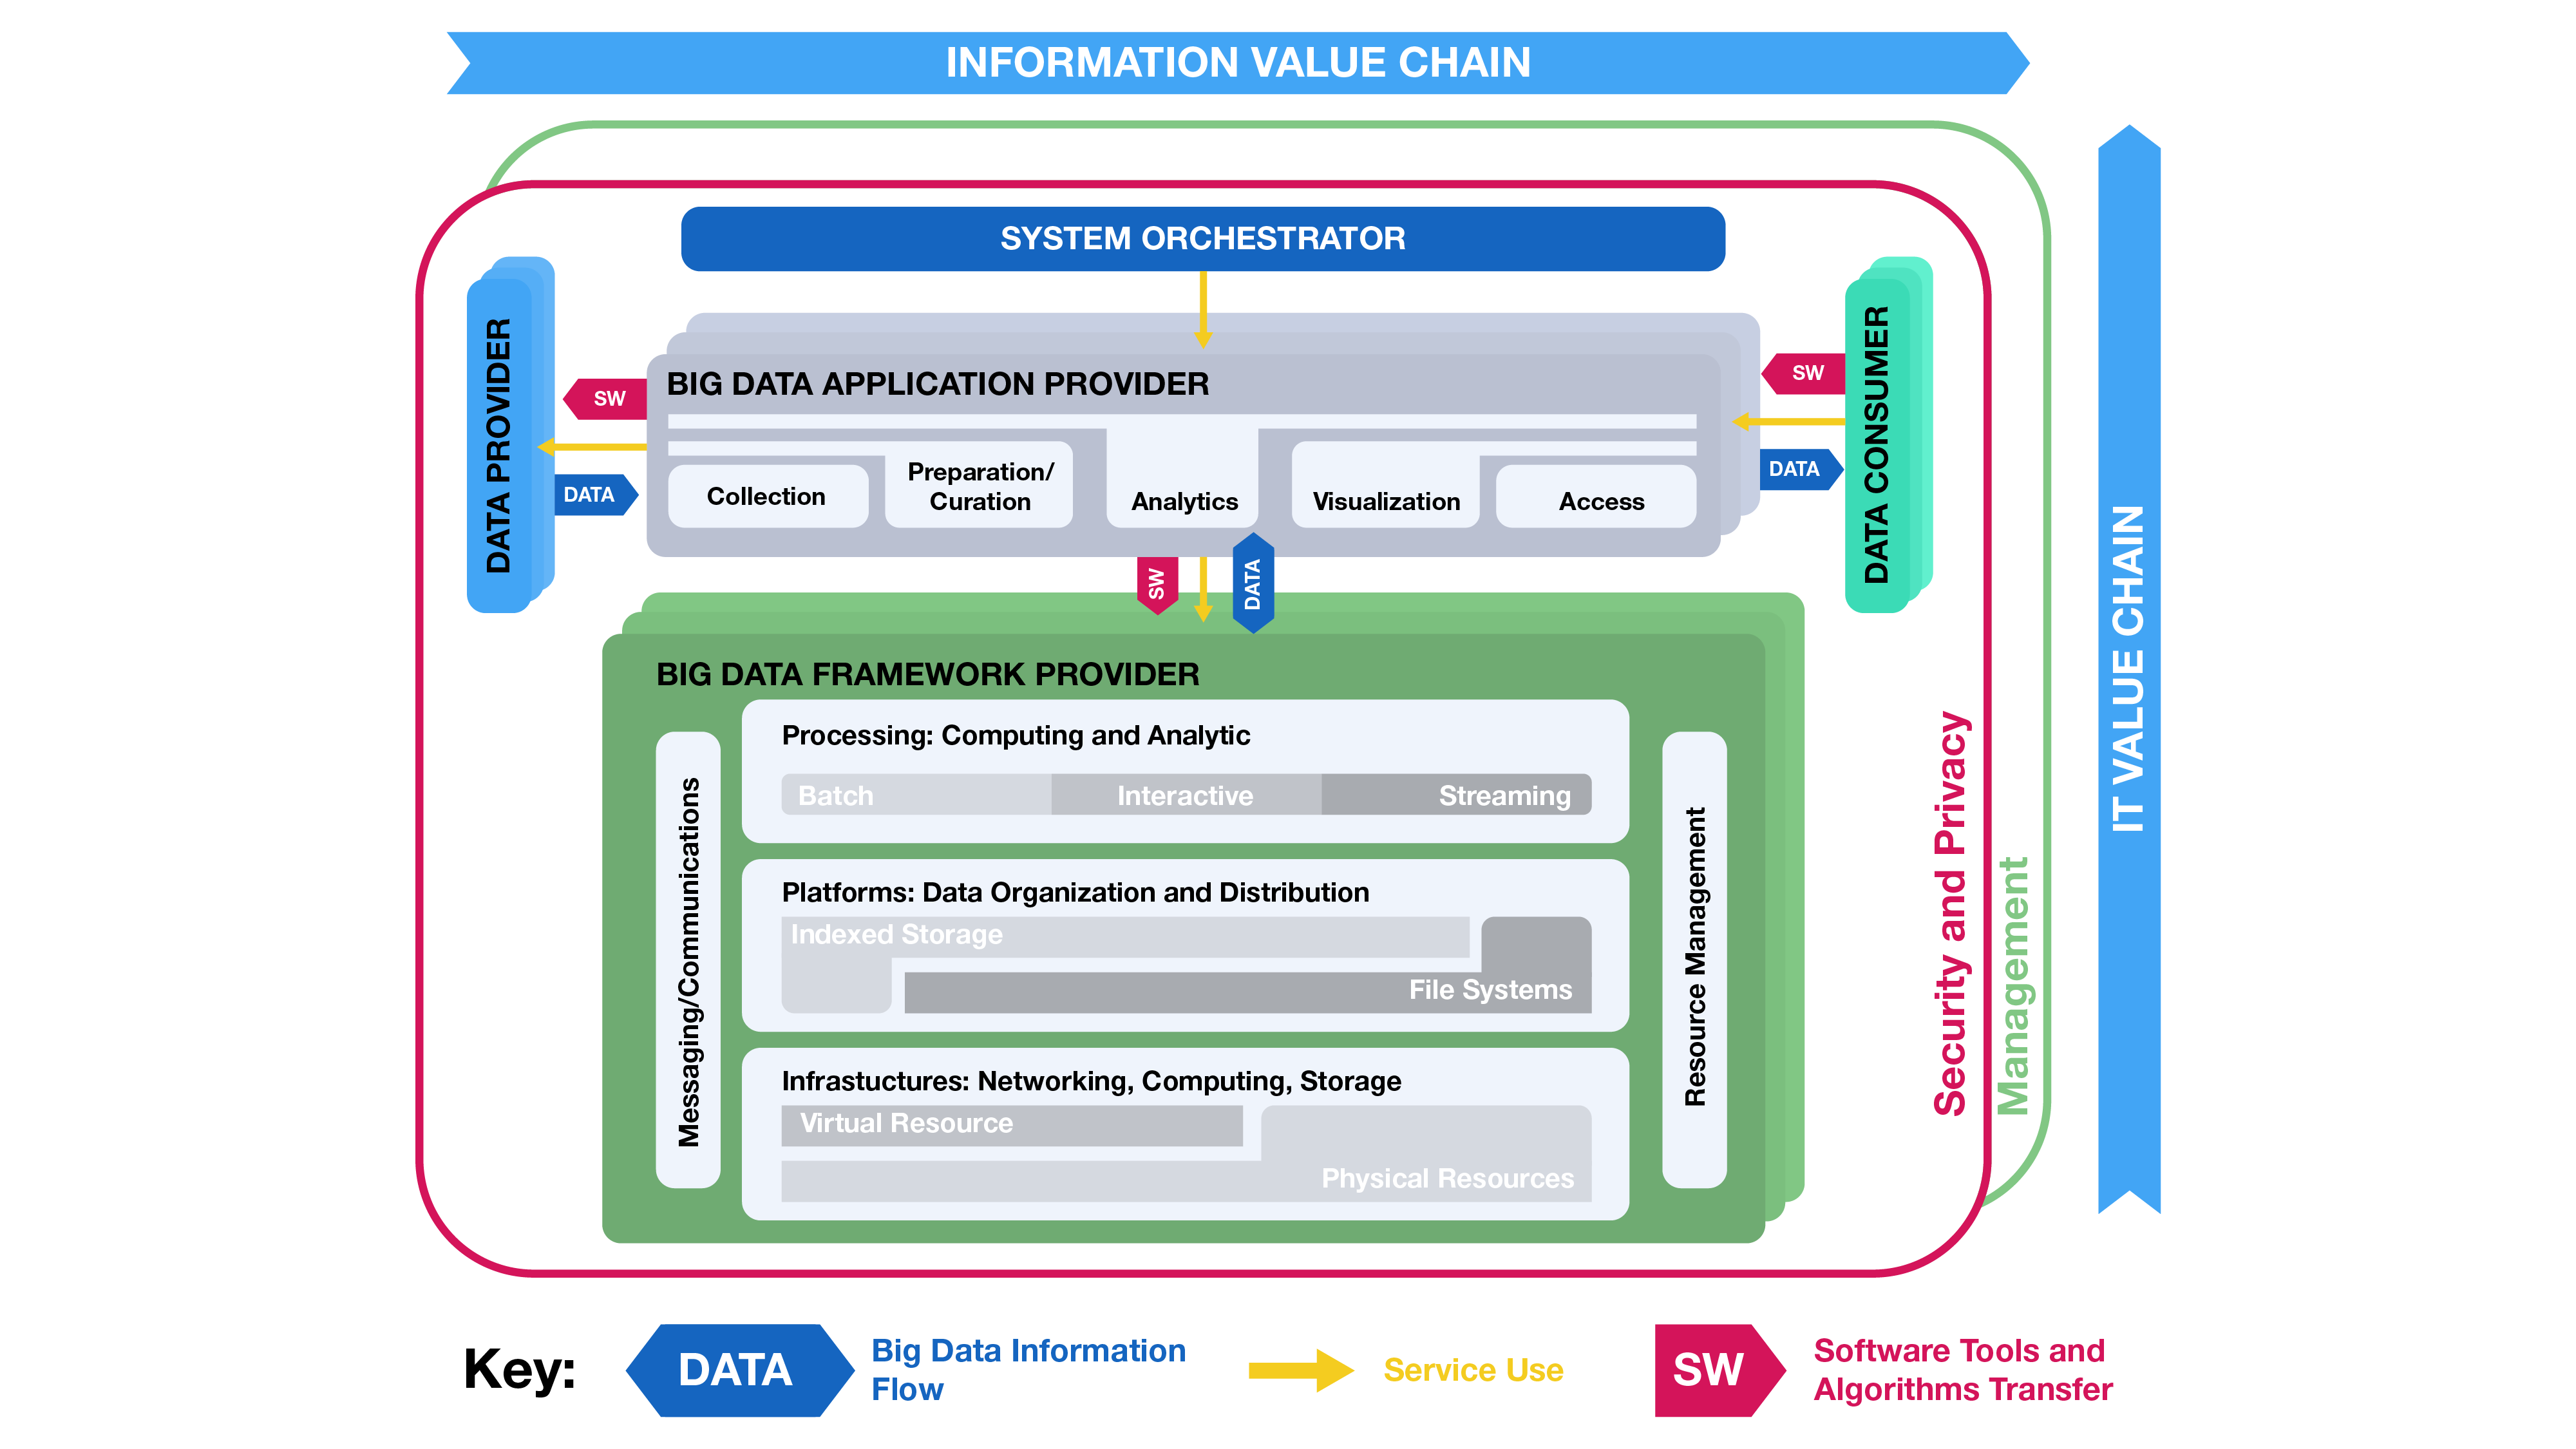
\includegraphics[width=18cm,height=8cm]{imgs/NBDRA_model}
	\caption{NBDRA Conceptual Model}
	\label{fig:NBDRA}
\end{figure*}
I 5 ruoli principali sui 2 assi dei Big Data abbiamo:

\subsubsection{System Orchestrator}
Il system orchestrator coinvolge spesso anche Information Value chain, poiché si preoccupa di implementare e monitorare i processi business a livelli enterprise e le varie politiche sui dati: Redere i dati accessibili per un tempo limitato oppure fornire i dati a velocità diversa(passando il dato in memoria al disco).
Può assegnare/fornire componenti framework fisici o virtuale al sistema, questa assegnazione può essere molto spesso elastica ed indipendente.
Può fornire supporto GUI e collegare i varie applicazioni a un livello alto, e attraverso il management fabbric monitorare i carichi e il sistema per garantire/specificare la qualità del servizio necessaria per i vari carichi.
E' molto spesso centralizzato.
Es. Ambari/Cloudera

\subsubsection{Data Provider}
Può essere sia un software (ad es. in una pipeline più grande) che una persona. Se è una persona metterà i suoi dati e userà gli strumenti di collection e curation/preparation per caricare i dati sul sistemi e migliorarne la qualità, Se un software metterà is suoi dati a disposizione attraverso delle interfacce come Apache Scoop. 
Il data provider può essere interno o esterno alla piattaforma, deve fornisce i diritti di accesso ai dati, ed è obbligato a seguire le policy di privacy e security fabbric. 
I dati possono essere inseriti in pull o push.
es. Flume per caricare i dati da MySQL a HDFS.

\subsubsection{Data Consumer}
Riceve i output dei sistemi BigData, può anche lui fare pull e push dei dati, può usarli le informazioni per data reporting, retrival/search e visualization. Ci deve essere l'autenticazione ed autorizzazione daparte della privacy and security fabbric per la comunicazione tra l'architettura e il Data Consumer.

\subsubsection{Big Data Application Provider}
Corrisponde alle attività tipiche di un Data Scientist, che esistono anche nei sistema tradizionali ma hanno delle trasformazioni nella implementazioni con i Big Data. Queste attività sono:
\begin{myitemize}
	\item Collection: Si occupa di gestire l'interfaccia fornita dal Data Provider, salva/gestisce questi dati in una certa zona affinché questi non vengano persititi, inoltre implementa funzionalità di estrazione dati dal data provider;
	\item Preparation: Effettua Data Validation, rimozione outlier, standardizzazione, formattazione e arricchimento. 
	Cerca di promuovere dati di alta qualità;
	\item Analytics: Estrazione conoscenza dai dati, sfruttando il software sottostante del Big Data Framework Provider;
	\item Visualization: Presentazione dati in maniera visuale;
	\item Access: E' l'opposto della collection, si preoccupa di esporre i dati verso l'esterno. 
\end{myitemize}

\subsubsection{Big Data Framework Provider}
Fornisce le infrastrutture per supportare i Big Data Application Provider. Si occupa in particolare di:
\begin{myitemize}
	\item Processing dei dati - ha una dualità: da una parte è un framework che mette a disposizione delle interfacce per la programmazione per fare certe cose (es. MapReduce) e dall'altra parte definisce come l'implementazione viene effettuata. I framework possono variare tra un proccessamento batch e in streaming.
	\item Platforms per l'organizzazione e immagazzinamento dei dati - può contenere i meta-dati insieme alle descrizione semantiche dei dati. 
	Può essere relazionale distribuito o non relazionale.
	\item Infrastructures per l'esecuzione fisica del nostro software, è l'insieme delle risorse computazionali fisiche o virtuali sulle quali il nostro sistema Big Data gira, può essere costituito da server di grandi o piccole dimensione. 
	Queste componenti forniscono:
	\begin{myitemize}
		\item Networking - Possono essere definiti attraverso software e possono essere reti fisiche che può essere a sua volta partizionato in reti virtuali. 
		Possono essere reti puramente virtualizzate cioè tutto quanto (firewall, router, load balancing) sono realizzate in maniera virtuale (es. VM dentro la nostra macchine);
		\item Computing - Hardware, Software, OS, memoria per il computing;
		\item Storage - dischi per storare (in locale), RAID, in rete ecc.
		\item e altri servizi come il Raffrendamento, l'apparto elettrico e la sicurezza
	\end{myitemize}
	Può essere deployato su ambienti fisici che virtualizzati (nativi, hostati o contenerizzati).
\end{myitemize}
Inoltre ha 2 ruoli diffusi nelle 3 componenti sopraindicate:
\begin{myitemize}
	\item Comunicazione e messaggistica tra le componenti;
	\item Gestione delle risorse per l'integrazione delle componenti.
\end{myitemize}

\subsection{I 2 ruoli diffusi per Big Data}
questi 2 ruoli prendono il nome di Fabric, il termine Fabric(tessuto) viene usato perché queste 2 ruoli cross-cutting, cioè sono presenti un pò ovunque nell'architettura.

\subsubsection{Management fabbric}
Le due attività principali associate:
\begin{myitemize}
	\item Gestione del sistema per provvedere le risorse, gestione dei software e pacchetti e infine la gestione delle configurazioni e performance delle varie pipeline;
	\item Ciclo di vita dei Big Data, BDLM (Big Data Life Cycle Management), contiene l'enforcing delle Policy (es. encoding/decoding), gestione dei meta data (data governance), accessibilità dei dati, data recovery e la loro preservazione.
\end{myitemize}


\subsubsection{Security and Privacy Fabric}
Si occupa delle tre caratteristiche tipiche delle security: 
\begin{myitemize}
	\item Autenticazione: Indica tutte le attività che validano l'utente;
	\item Autorizzazione: Una volta autenticato l'utente verifica i suoi permessi, es. alcuni dati potrebbero non essere accessibili a certi utenti;
	\item Auditing: riguarda la registrazione degli eventi che accadono nel sistema, può far partire un allarme in caso di evento anomalo o a posteriori analizzare la sequenza di eventi (con i file log).
\end{myitemize}

\section{Virtualizzazione}
Per i computer sono stati definiti con le 5 componenti classiche:
\begin{myenumerate}
	\item Input Devices: Tastiera ecc.
	\item Output Devices: Display ecc.
	\item Storage Devices: Volatile(RAM), Permanente(HD, SSD)
	\item Processore:
	\begin{myitemize}
		\item Datapath
		\item Control
	\end{myitemize}
	\item Network
\end{myenumerate}
La virtualizzazione permette l'esecuzione di più sistemi operativi simultaneamente sulla macchina in maniera totalmente isolata. 
Può essere visto come una emulazione di un software o hardware su cui altri software possono eseguirsi, questo ambiente emulato è detto virtual machine.
Il concetto di VM è stato sviluppato negli anni 60 da IBM sui mainframes.
Viene abbandonato con la nascita di PC moderni e ripreso con la crescita recente di cloud. La virtual machine viene ottenuto attraverso un Virtual Machine Monitor detto anche ipervisore.\\
L'\textbf{Hypervisor}(Ipervisore) è un software che giace sotto gli OS virtualizzati per offrire le funzionalità di condivisione delle risorse disponibili in modo tale che il programma o OS in esecuzione veda queste risorse come se fosse a lui dedicate. 
Le risorse sono CPU, memoria, storage e la rete.\\
Vi sono diversi benefici della virtualizzazione:
\begin{myitemize}
	\item Visione unificata delle risorse es. vedo tanti dischi come un unico disco;
	\item Consolidazione delle risorse virtualizzate, in modo da avere l'ottimo utilizzo delle risorse;
	\item Facilità di implementare la ridondanza per copiare gli ambienti virtualizzati;
	\item Facilità la migrazioni di sistema su un altro, inoltre se non cambio ipervisore la macchina(virtuale) funzionerà identicamente a prima;
	\item Gestione centralizzata del hardware e software.
\end{myitemize}
Altri benefici/proprietà della virtualizzazione sono:\\
\textbf{Workload Isolation:} attraverso la virtualizzazione è possibile isolare completamente i programmi, che ha miglioramenti anche nella sicurezza, inoltre aumenta affidabilità poiché il fallimento di un programma non comporta fallimento dei programmi poiché sono isolati, inoltre si risolvono anche i problemi riguardanti i conflitti di librerie in questo modo. Infine si ottiene un controllo sulle performance poiché l'esecuzione di una VM non affligge il performance dell'altra;\\
\textbf{Workload Migration:} ciò aiuta in:
\begin{myitemize}
	\item Mantenimento di Hardware;
	\item Load Balancing;
	\item Fault Tolerance;
	\item Disaster Recovery.
\end{myitemize}
Poiché possiamo spostare tutto l'ambiente virtualizzato su una nuova macchina in maniera abbastanza trasparente, per fare ciò la macchina dovrebbe essere sospesa, totalmente serializzata per essere inviata nella rete, migrata su una nuova macchina e fatta ripartire immediatamente o solo salvata senza esecuzione.\\
\textbf{Consolidazione:} Sfruttando il Workload Migration è possibile consolidare macchine separate su un unica piattaforma riducendo i costi (usata molto spesso nei Datacenter in orari non di picchi).\\
\begin{figure}[h]
	\centering
	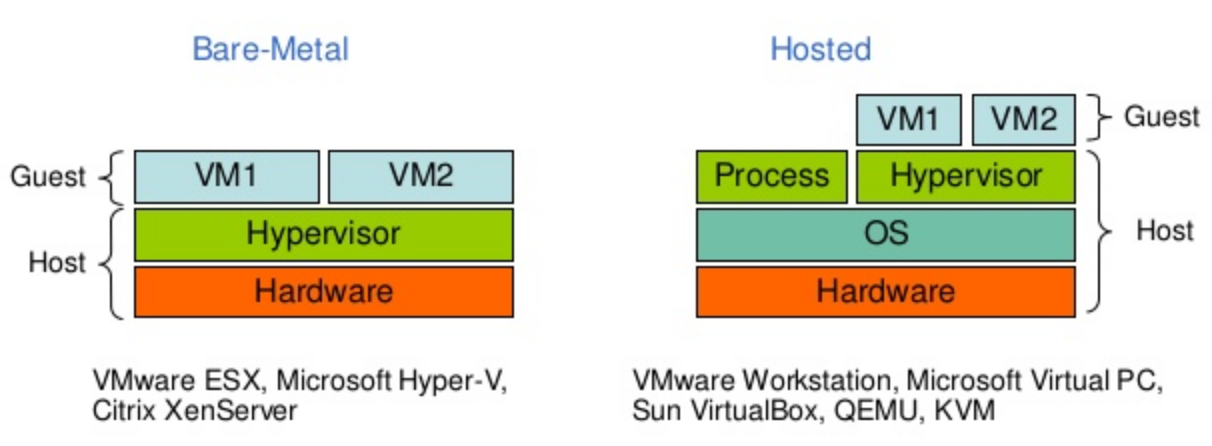
\includegraphics[width=\linewidth]{imgs/hypervisor_type.png}
	\caption{I tipi di Hypervisor}
	\label{fig:hypervisor_type}
\end{figure}
I diversi tipi di HyperVisor sono (Fig \ref{fig:hypervisor_type}):
\begin{myitemize}
	\item \textbf{Hosted}: in questo caso ipervisore è un processo che gira al di sopra del sistema operativo e permette l'esecuzione di più macchine Guest.
	In questo caso quindi bisogna installa prima un OS su cui verrà installa VMM (ipervisore) e adesso l'host potrà eseguire le applicazioni all'interno della sua finestra.
	Il vantaggio qua è la facilità di installazione e configurazione, inoltre la HostOS e GuestOS sono non modificati e non dipendono dal particolare hardware, ma gli svantaggi sono la degradazione delle performance e la mancanza di supporto real time OS poiché vi sono varie entità/software in mezzo;
	\item \textbf{Bare-Metal}: in questo caso ipervisore funziona direttamente al di sopra del Hardware.
	In questo caso l'ipervisore è un OS molto leggero e comunica direttamente con hardware al posto di dipendere su un altro OS. 
	I vantaggi sono miglioramento in I/O e supporto real time, mentre gli svantaggi sono la difficoltà di istallazione e configurazione e la dipendenza dal tipo di hardware specifico.
\end{myitemize}
Ci sono principalmente 2 tecniche di virtualizzazione: \textbf{Software Virtualization} (di cui abbiamo parlato fino ad adesso) e \textbf{Hardware Assisted Virtualization}.\\
Nella \textbf{Virtualizzazione Totale} VMM si preoccupa di emulare in maniera completa tutto l'hardware, quindi avremo un processore, memoria, disco e network virtuale.
in questo caso OS ospite non è consapevole dell'esistenza dell'ambiente virtuale e ogni macchina è del tutto indipendente.
A livello CPU, avviene la traduzione binaria: Questo avviene in diversi anelli di sicurezza, in particolare sono 4, dove l'anello 0 è quello più privilegiato e permette l'esecuzione del codice direttamente sul hardware e qua dove viene eseguito il kernel dell'OS.
Le applicazione dell'utente vengono eseguite sull'ultimo anello (anello 3).\\
L'ipervisore gira sull'anello 0 mentre le GuestOS gira sull'anello 1, quindi hanno più permessi delle normali applicazioni. 
VMM ha accesso sul anello 0 per avere accesso diretto sulla CPU piuttosto che virtualizzarla. \\
La \textbf{Para-Virtualizzazione} ha un approccio diverso rispetto alla virtualizzazione totale (è una via di mezzo tra total virtualization e bare-metal), in questo caso il Guest sono consapevoli della VMM e usa chiamate speciali in alcuni casi per essere eseguite direttamente sul hardware e ciò comporta un miglioramento nella performance ma ciò lo rende meno flessibile.\\
La \textbf{OS-level Virtualization (Containerization)} non usa la VMM, la virtualizzazione è fornita direttamente dal HostOS che esegue tutte le funzioni di un ipervisore totalmente virtualizzato, quindi ha una partizione puramente virtuale delle risorse, e ciò comporta un'assegnazione flessibile delle risorse alle varie applicazioni. Es. Docker.\\
Ci sono 3 modelli di servizio:
\begin{myenumerate}
	\item \textbf{Server Virtualization}: supponiamo di avere diversi server su macchine diverse, in caso di un problema (crash di un nodo) o vi è un bisogno di upgrade, in caso di macchine fisiche dovrò prendere lo stesso modello o lo stesso vendore, la soluzione è quella di sfruttare una medesima macchina con un virtualizzatore e mettere i diversi server insieme.
	In questo modo ho una consolidazione, risorse condivise, una gestione centralizzata, facilità di migrazione, maggiore ROI e meno spazio occupato.
	La Disaster Ricovery e scalabilità viene facilitata, diversi modelli a scelta (basta che sia uguale l'ipervisore), ho maggiore disponibilità.
	\item \textbf{Desktop Virtualization}: è la tecnologia che separa l'ambiente desktop e le applicazione software dal cliente fisico che lo usa. 
	Il nostro desktop diventa un thin client che usa PC privo della memoria RAM e potenza calcolo necessaria per far funzionare una macchina reale, la macchina gira su un pool di VM su un server su un data center.\\
	I benefici sono molteplici: Upgrade di software e OS facilitato, alta disponibilità, fault tolerance, accessibile da LAN, WAN, Internet, inoltre vi è la possibilità di far eseguire una piccola parte della computazione dal dispositivo locale.
	\item \textbf{Application Virtualization}: Molto simile alla Desktop virtualizzazione, solo che al posto di tutto il desktop, sono le applicazione ad essere in virtualizzate, quindi un applicazione che gira sul desktop, fa la computazione sul cloud, una piccola parte della computazione può essere effettuata anche in locale.
	I vantaggi sono molto simili a quelli del Desktop Virtualization, un vantaggio aggiuntivo può essere che pago solo quello che uso, riducendo i costi delle licenze.
\end{myenumerate}
%\section{Lezione 3 - 09/10}

\section{Cloud}
Cos'è il cloud? La possibilità di avere accesso alle risorse computazionale attraverso la rete on-demand ed è composto da 5 punti chiave, 3 modelli di servizio e 4 modelli. 
\\
Definizione ``vera'' del cloud secondo NIST: è un tipo di servizio distribuito di sistemi interconessi e computer virtualizzati dinamicamente provisionati e presentati come un unica risorsa computazionale basato su service-level agreement.
\\
I tre modelli del servizio sono:

\begin{myenumerate}
	\item IaaS Infrastructure as a service es. le macchine virtuali
	\item PaaS Platform as a service, ci viene fornito una scatoletta dove eseguire/testare le applicazioni, il provider sarà il garante del fatto che il sistema sia abbastanza responsive e abbia un runtime sufficiente.
	\item Saas Software as a service, es. GMail quindi utente non può fare niente tranne usare il software.
\end{myenumerate}
Le 5 caratteristiche che identificano il cloud sono:
\begin{myenumerate}
	\item Scalabilità, Elasticità:
	\begin{myitemize}
		\item Scalabilità è una proprietà del sistema di crescere in maniera graduale col crescere di richieste, può essere orizzontale o verticale.
		\item Elasticità è l'abilità di adattarsi automaticamente per inizializzare la scalabilità.
	\end{myitemize}
	Ciò si può ottenere attraverso provisioning dinamico, che è un ambiente complesso che permette la allocazione e disallocazione di applicazione o un console amministrativo.
	\item Disponibilità, Reliability:
	\begin{myitemize}
		\item Availibility è il rapporto tra il up-time e down-time
		\item Affidabilità è la capacità di funzionare in situazioni particolari
	\end{myitemize}
	Questi punti possono essere ottenuti attraverso:
	\begin{myitemize}
		\item Fault Tolerance
		\item Resilience
		La resilienza è l'abilità di ritornare allo stato di funzionamento dopo un caso di fallimento del sistema (ad es. viene a mancare l'elettricità).
		Quindi i sistemi devono avere le policy e procedure per il recupero, ad es. Backup (dei dati off-site oppure di tutto il sistema) oppure preparazione per fault come un una corrente non-interrompibile (UPS) oppure insurghi di corrente.
		\item Sicurezza
		La sicurezza riguarda 
		\begin{myitemize}
			\item la protezione i dati, mantenendo l'accesso ai dati riservato solo in base ai privilegi
			\item 
		\end{myitemize}
	\end{myitemize}
	\item Gestibilità, Interoperabilità:
	La Gestbilità riguarda la gestione di questi sistemi mentre la interoperabilità è una proprietà di un prodotto o sistema per lavorare con altri prodotti.
	Lo si ottiene attraverso system monitoring che è un processo che monitora lo stati dei hardware, metriche dei performance, i log dei sistemi, il pattern dei accessi alla rete ecc. Ed è importante anche il sistema Billing.
	Il Load balancing è una tecnica per la distribuzione del workload su un sistema di computer, CPU, HD or altre risorse per ottenere l'utilizzo ottimale, migliorando così: l'utilizzo del sistema, la performance e l'efficienza energetica.
	\item Accessibilità, Portabilità
	
	\item Ottimizzazione della performance
\end{myenumerate}
Da un punto di vista dell'utente, lui non vuole sapere come e cosa viene fatto né chi gestisce il servizio, ma vuole solo un servizio funzionale.

SOA, Service Oriented Architecture, è un insieme di servizio poiché non basta di solito un servizio per implementare un servizio web per clienti.

SLA, Service Level Agreement è un contratto tra il service provider e il cliente che specifica il livello di servizio che il service provider deve fornire in termini di QoS.
Le metriche più comuni sono up-time e down-time, Response time.

\section{Lezione 4 - 15/10}
IaaS fornisce automaticamente il processing, storage, network e altre risorse fondamentale per il computing, e l'utente può installare i software che sono per lui necessari.
\\
L'utente ha accesso a due interfacce:
\begin{itemize}
	\item Inerfaccia per gestione delle risorse, queste risorse sono:
	\begin{itemize}
		\item VM: creazione, cancellazione, gestione, sospensione delle VM 
		\item Virtual Storage:
		\item Virtual Network: gestione delle IP associate ecc.
	\end{itemize}
	\item Interfaccia del il monitoring del sistema: viene messa a disposizione da VIM: L'orchestrazione delle macchine su un server viene gestita dalla Virtual Infrastructure Mangaser(VIM), diverse metriche vengono usate per il monitoraggio es:
	\begin{itemize}
		\item VM: CPU usage, memory usage
		\item Virtual Storage: utilizzo del disco
		\item Virtual Network: L'uso della banda ecc.
	\end{itemize}
\end{itemize}
 
PaaS mette a disposizione all'utente i lunguaggi di programmazione e i tools (come IDE) supportati dal provider, ma il controllo sul deployement dell'applicazione non è in mani del consumer...
\\
alla base vi è una archittettura come quella di IaaS, offrono i Programming IDE e le API supportati dall'ambiente, spesso hanno in comune le funzioni come: computation e lo storage.
\\
L'interfaccia messa a disposizione è quello per il controllo del sistema per:
\begin{itemize}
	\item Policy based control: le azioni seguono delle regole per prendere delle decisioni quindi azioni seguite con if <> then <>
	\item Controllo del workflow: descrizione del flusso di installazione e configurazione delle risorse oppure dei daemon.
\end{itemize}

SaaS: vengono fornite al cliente applicazione del provider in cloud, l'utente non può gestire lo sviluppo dell'applicazione ma può interagire con esso attraverso ad es. portali web, che con introduzione del Web 2.0 ha potenziato l'iterabilità con l'applicazione in cloud, es: Facebook(Messenger), Office, Skype, sistema CRM, sistema medico nazionale, sistema di trasporto pubblico.

I 4 modelli primari di un modello cloud sono:
\begin{itemize}
	\item Public Cloud: L'infrastruttura viene messa a disposizione del pubblico or organizzazioni grandi attraverso pagamento per il suo uso, le caratteristiche sono:
	\begin{itemize}
		\item Infrastruttura omogenea per garantire le medesime prestazioni a due utenti che pur trovandosi in posti diversi usano lo stesso servizio
		\item Policy customizzate
		\item Risorse dedicate
		\item In-house managed infrastructure? errore
		\item End-to-end control? errore
	\end{itemize} 
	\item Private Cloud:
	A differenza del public cloud l'hardware può essere eterogenea per via del costo e dal fatto che una azienda privata non butta via un hardware solo per averli omogenea.
	\item Community Cloud: è una struttura gestita da diverse entità, in pratica più entità mettono insieme i loro cloud privati per generare un super cloud, ad esempio alcune università americane possono unire i loro cloud per qualche ricerca ecc.
	\item Hybrid Cloud: è la comoposizioni di più tipi di cloud, ad esempio un azienda privata crea il suo cloud privato per la gestione di informazioni sensibili e usa l cloud pubblico per il resto, oppure per la scalabilità in caso i traffico aumentato.
\end{itemize}

\subsection{Amazon ECOSYSTEM}
Amazon Web Service sono creati per lavorare indipendentemente ma lavorano bene anche tra di loro: condividendo tra di loro le stesse convenzioni di nomi e autenticazione e minimizzando le connessioni interne.
\\
Amazon mette a disposizione il concetto di regione e di zona disponibile:
\begin{itemize}
	\item Ciascuna Availibility zone è un data center indipendente con la propria griglia di potenza e connessione della rete, le zone all'interno di una regione sono collegate tra di loro attraverso connessione a latenza bassa.
	\item Regione è un cluster di data center localizzati in una area geografica. 
	Le zone vengono create per la massima fault tolerance e stabilità.
\end{itemize}
Esiste AWS GovCloud che è una regione AWS isolata.\\
Simple Storage Service (S3) è una storage object che è un sistema di archiviazione piatto cioè non è possibile creare cartelle al suo interno, i dati salvati su S3 vengono distribuite automaticamente. 
S3 sta alla base fi tutta l'infrastruttura che sta alla base di amazon e-commerce.
Oltre a S3 amazon fornisce anche un EBS (Elastic Block Store), questo disco può essere formattato, montato e usando come hard disk locale, è un volume che persiste indipendentemente dal resto.\\

EC2(Elastic Cloud Computing)
i concetti chiave che constituiscono EC2:
\begin{itemize}
	\item Amazon Machine Image (AMI):
	contiene il sistema operativo e eventuali software, possono essere pre-built, create, modificate e vendute. Ciascun AMI ha un ID unico.
	\item Istanza: rappresenta una copia di AMI in esecuzione, multiple copie di un unica AMI può essere messa in esecuzione
	\item Elastic IP address: allocazione di un IP statico e collegarle alla propria istanza; 
\end{itemize}
I core messi a disposizione dal server vengono virtualizzati sui separando i core che dividendo il core-time. L'unità di misura è EC2 Compute units che corrisponde a Intel Xeon a 1.0-1.2 GHz 2007.\\
Le risorse possono essere persistenti cioè anche in caso di fallimento del hardware Amazon ci garantisce la sua persistenza oppure risorse ephimere cioè l'utente deve garantire la sua ridondanza e mantenimento come HardDisk, mentre le componenti persistenti sono:
\begin{itemize}
	\item Elastic IP Address
	\item EBS
	\item 
\end{itemize}

I modelli del prezzo sono:
\begin{itemize}
	\item On demand
	\item Reservati
	\item Spot (Asta)
\end{itemize}

\section{Lezione 5 - 16/10}
AutoScaling avviene per via dei trigger di solito sui utilizzo CPU/memory, l'auto scaling può avvenire sia per scale in che scale out all'interno di un scale group (max min) pre-definito. Una macchina può essere o spenta o terminata, nel caso viene terminata viene eliminata completamente.
Le metriche più usate per il cloudWatch sono
\begin{itemize}
	\item CPU usage
	\item Latenza
	\item Numero di Richieste
	\item Il numero di Host(macchine) in buona salute
	\item Il numero di macchine che non stanno funzionando benissimo
\end{itemize}
In generale almeno due trigger sono necessari per mantenere un equilibrio desiderato.
Un allarme è una metrica e verifica se questa metrica supera un limite stabilito per un certo tempo.
Quindi per creare un allarme è necessario specificare:
\begin{itemize}
	\item Metrica da osservare
	\item Il threshold della metrica
	\item Il numero di periodo di valutazione
\end{itemize}
Gli stati in cui la metrica si può trovare sono:
\begin{itemize}
	\item Ok, tutto bene!
	\item Alarm
	\item Insufficient data
\end{itemize}
Se l'allarme cambia lo stato e vi rimane per un determinato periodo di valutazione, un'azione viene invocata.

I scenari automatici dell'auto scaling sono:
\begin{itemize}
	\item Fleet Management: assicura il performance come dovrebbero, se un'istanza dovesse terminare questa viene individuata e si fa partire un'altra macchina. la determinazione della salute avviene con Health Check.
	\item Scheduled scaling: 
	\item Scaling Dinamico
\end{itemize}




i canditati per autoscaling sono:
\begin{itemize}
	\item Web Tier
	\item Application Tier
	\item Load Balancing Tier
	\item Stateless Tier
\end{itemize}

I sistemi di database di NoSQL, cache distribuito non sono fatti per auto scalare.

\end{document}
